\documentclass{beamer}
%\documentclass[11pt, handout]{beamer}

\usepackage{graphicx}
\usepackage{xspace}
\usepackage{tikz}
\usepackage{circuitikz}
\usepackage{hyperref}
\usepackage{adjustbox} 
\usepackage{protocolj}
\usepackage{multirow}
\usepackage{longtable,booktabs,setspace} 
\usetikzlibrary{shapes.geometric, arrows}

%% Alex L's macros 
%% taken and co-opted from a variety of sources
%
%% generic commands
%\newcommand{\NN}{\mathbb{N}}
%\newcommand{\RR}{\mathbb{R}}
%\newcommand{\compindist}{\approx_C}
%
%% definition counter
%\newcounter{defcounter}
%\setcounter{defcounter}{0}
%\newenvironment{definition}{\medskip\noindent\refstepcounter{defcounter}{\bf Definition \thedefcounter}\hspace*{2pt}}{\hspace*{\fill}\nopagebreak[4]$\diamondsuit$\medskip}  
%
%% block quote
%\newenvironment{blockquote}{%
%  \par%
%  \medskip
%  \leftskip=4em\rightskip=2em%
%  \noindent\ignorespaces}{%
%  \par\medskip}
%
%% Author Macros -- colors: red, magenta, blue, orange
%\newcounter{al}
%\newcommand{\al}[1]{\textcolor{blue}{\{AL-\arabic{al}: #1\}}\addtocounter{al}{1}}
%\newcounter{cat}
%\newcommand{\cat}[1]{\textcolor{magenta}{\{CAT-\arabic{cat}: #1\}}\addtocounter{cat}{1}}
%\newcommand{\ignore}[1]{}
%
%% From CompGC paper
%%\renewcommand{\sim}{S}
%%\newcommand{\Input}{\ensuremath{\textsf{Input}}\xspace}
%%\newcommand{\Output}{\ensuremath{\textsf{Output}}\xspace}
%%\newcommand{\Inputs}{\ensuremath{\textsf{Inputs}}\xspace}
%%\newcommand{\Outputs}{\ensuremath{\textsf{Outputs}}\xspace}
%%\newcommand{\Components}{\ensuremath{\textsf{Components}}\xspace}
%
%\newcommand{\Gates}{\text{Gates}}
\newcommand{\C}{\sf {C}}
\newcommand{\GC}{\sf {GC}}
%\newcommand{\AllInputLabels}{\sf {AllInputLabels}}
%\newcommand{\InputLabels}{\sf {InputLabels}}
%\newcommand{\InputWires}{\text{InputWires}}
%\newcommand{\OutputWires}{\text{OutputWires}}
%\newcommand{\Wires}{\text{Wires}}
%\newcommand{\A}{\mathcal{A}}
%\newcommand{\OT}{\textsf{OT}} % or mathsf
\newcommand{\Enc}{\textsf{Enc}} % or mathsf
\newcommand{\Dec}{\textsf{Dec}}
\newcommand{\Gen}{\textsf{Gen}}
\newcommand{\EncInv}{\Enc^{-1}}
\newcommand{\EncDKC}{\textsf{EncDKC}}
\newcommand{\DecDKC}{\textsf{DecDKC}}
\newcommand{\EncDKCInv}{\EncDKC^{-1}}
%\newcommand{\compIndist}{\approx_D}
%\newcommand{\outputrv}{{\sf output}}
%\newcommand{\viewrv}{{\sf view}}
\newcommand{\CompGC}{\textsf{CompGC}\xspace}
%\newcommand{\JustGarble}{\textsf{JustGarble}\xspace}
%\newcommand{\Naive}{\textsf{Naive}\xspace}
%\newcommand{\scmc}{SCMC\xspace} % Single Communication Multiple Connnection


\renewcommand<>{\item}[1]{\only#2{\beameroriginal{\item}{#1}}}
    \mode<presentation> {
        \usetheme{default}
        \usecolortheme{seahorse}
        \setbeamertemplate{footline}[page number] 
        \setbeamertemplate{navigation symbols}{} 
    }

    \title[Short title]{Implementing Component-Based Garbled Circuits\\
    } 
    \author{Alex Ledger} 
    \institute[Reed College]{
        Reed College \\ 
    }
    \date{\today}

    \begin{document}

    \begin{frame}
        \titlepage 
    \end{frame}

    \begin{frame}
        \frametitle{Overview}
        \begin{enumerate}
            \item Cryptographic Primitives
            \item Security and Classical Garbled Circuits
            \item Improvements to Garbled Circuits
            \item Component-Based Garbled Circuits + SCMC
            \item Implementation and Results
        \end{enumerate}
    \end{frame}

    \begin{frame}
        \frametitle{Introduction}
            TODO
    \end{frame}

    \begin{frame}
        \frametitle{The Millionaire Problem}
        \begin{itemize}
            \item Alice and Bob wish to determine who is wealthier.
            \item They do not want to disclose their wealth to each other.
                \begin{itemize}
                    \item Alice has \$$x$, Bob has \$$y$.
                    \item Alice should not learn anything about $y$.
                    \item Bob should not learn anything about $x$.
                \end{itemize}
        \end{itemize}
        \begin{equation}
            f(x,y) = \left\{
                \begin{array}{ll}
                    Alice, & \quad y \leq x; \\
                    Bob, & \quad y > x.
                \end{array}
                \right.
        \end{equation}

            \begin{figure}
                \centering
                \includegraphics[scale=0.8]{images/setup}
            \end{figure}
            % http://www.alexirpan.com/2016/02/11/secure-computation.html
    \end{frame}

        \begin{frame}
            \frametitle{Security Parameter}
            \begin{itemize}
                \item asdf
            \end{itemize}
        \end{frame}

        \begin{frame}
            \frametitle{Encryption}
                \begin{align*}
                    \label{eqn:encryption}
                    \begin{split}
                        \Gen(1^n) & \rightarrow k \\
                        \Enc_k (pt) & \rightarrow ct  \\
                        \EncInv_k(ct) & \rightarrow pt
                    \end{split}
                \end{align*}
        \end{frame}

        \begin{frame}
            \frametitle{Security of Encryption}
            An encryption scheme is secure under a chosen-plaintext attack if for all probabilistic polynomial-time adversaries $A$, there exists a negligible function $\mu$ such that
            \begin{align*}
                Pr[E_{\A, \Pi}(n) = 1] \leq \frac{1}{2} + \mu(n)
            \end{align*}
            where $E$ is the following experiment:
            \begin{enumerate}
                \item Generate key $k$ by running $\Gen(1^n)$. 
                \item The adversary $\A$ is given $1^n$ and oracle access to $\Enc_k$, and outputs a pair of messages $m_0$ and $m_1$ of the same length.
                \item A uniform bit $b \samples \{0,1\}$ is sampled uniformly at random, and then ciphertext $c \gets \Enc_k(m_b)$ is computed and given to $\A$.
                \item Then $\A$ continues to have oracle access to $\Enc_k$, and outputs a bit $b'$. 
                \item The output of the experiment is defined to be $1$ if $b' = b$ and $0$ otherwise. If at any point $\A$ encrypts $m_0$ or $m_1$ with their encryption oracle, the output is $0$. $1$ indicates that the adversary wins, and $0$ indicates that the adversary loses.
            \end{enumerate}
        \end{frame}

        \begin{frame}
            \frametitle{Computational Indistinguishability}
            Intuition: 
            \begin{itemize}
                \item Let $\mathcal{X}$ and $\mathcal{Y}$ be distribution ensembles.
                \item Give an adversary one of the distribution ensembles.
                \item Can the adversary sample from the distribution a polynomial number of times to determine which distribution they were given?
            \end{itemize}

            Formal Definition:
            \begin{itemize}
                \item Let $\mathcal{X} = \{X_n\}_{n \in \NN}$ and $\mathcal{Y} = \{Y_n\}_{n \in \NN}$ be distribution ensembles.
                \item Then $\mathcal{X}$ and $\mathcal{Y}$ are computationally indistinguishable, denoted $\mathcal{X} \compindist \mathcal{Y}$, if for all probabilistic polynomial-time algorithms $D$, there exists a negligible function $\mu$ such that:
                    \begin{align*}
                        |Pr_{x \gets X_n} [D(1^n, x) = 1] - Pr_{y \gets Y_n} [D(1^n, y) = 1]| < \mu(n)
                    \end{align*}
            \end{itemize}
        \end{frame}

        \begin{frame}
            \frametitle{Boolean Circuits}
            \begin{itemize}
                \item We encode a function $f$ into a circuit $C$.
                \item Circuit $C$ is made of AND, XOR and NOT gates.
                \item Each gate has two input wires and a single output wire
            \end{itemize}
            \begin{figure}
                \centering
                \includegraphics[scale=0.6]{images/less_than}
            \end{figure}
        \end{frame}

        \begin{frame}
            \frametitle{Oblivious Transfer (OT)}
            \begin{itemize}
                \item Alice potentially sends either $m_0$ or $m_1$ to Bob.
                \item Bob, without seeing $m_0$ or $m_1$, decides that he wants $m_b$.
                \item Bob receives $m_b$.
                \item Property 1: Alice does not know which message Bob recieved.
                \item Property 2: Bob doesn't anything about $m_{1-b}$.
            \end{itemize}

            \begin{figure}
                \includegraphics[scale=0.6]{images/ot}
            \end{figure}
        \end{frame}

        \begin{frame}
            \frametitle{Oblivious Transfer 2}
            \begin{figure}
                \centering
                \includegraphics[scale=0.5]{images/ot_details}
                % https://www.codechef.com/problems/OBLIVI
            \end{figure}
            RSA-based oblivious transfer
        \end{frame}

        \begin{frame}
            \frametitle{Setting up Security of 2PC}
                \begin{itemize}
                    \item Privacy of inputs
                        \begin{itemize}
                            \item Alice and Bob do not learn anything about the each other's input.
                            \item Except for info that is inferable from $x$ and $f(x,y)$.
                            \item Bob should not learn that $1,000,000 < x \leq 2,000,000$.
                            \item But if $y < x$ and $y = 2,000$, then he learns $x < 2,000$.
                        \end{itemize}
                    \item Correctness
                        \begin{itemize}
                            \item Alice and Bob receive $f(x,y)$.
                            \item As opposed to some value near $f(x,y)$.
                            \item Or not receiving a value at all
                        \end{itemize}
                \end{itemize}
        \end{frame}

        \begin{frame}
            \frametitle{Semi-Honest}
            \begin{itemize}
                \item We assume that each party obeys the protocol, but attemps to learn extra information from its interactions
                \item In contrast, Alice and Bob could lie, deceive, not send some messages, etc. 
                    \begin{itemize}
                        \item This is called the malicious setting
                    \end{itemize}
                \item Reasons we use the semi-honest setting
                    \begin{itemize}
                        \item It's easier
                        \item Some realistic scenarios (e.g, hosptitals)
                        \item \JustGarble\,\,is written for semi-honest setting
                    \end{itemize}
            \end{itemize}
        \end{frame}

        \begin{frame}
            \frametitle{Security of 2PC (Overview)}
            \begin{figure}
                \centering
                \includegraphics[scale=0.25]{images/security}
            \end{figure}
            A secure computation protocol is secure if Alice and Bob learn the same information in the real world as they would in ideal world.
        \end{frame}

        \begin{frame}
            \frametitle{Security of 2PC (Ideal World)}
            \begin{itemize}
                \item We use computational indistinguishability
                \item Model information that Alice and Bob can infer in real and ideal world
                \item Simulators: adversaries in the real world
                    \begin{itemize}
                        \item We have $\sim_A$ and $\sim_B$
                        \item Take as input $x$ and $f(x,y)$.
                    \end{itemize}
                \item So our \textit{distribution ensembles} of information in the ideal world are
                    \begin{align*}
                        \{\sim_A(x, f(x,y)\}_{x \in \{0,1\}^*} \text{ and }
                        \{\sim_B(y, f(x,y)\}_{y \in \{0,1\}^*}
                    \end{align*}
            \end{itemize}
        \end{frame}

        \begin{frame}
            \frametitle{Security of 2PC (Real World)}
            \begin{itemize}
                \item In the real world, we introduce $\viewrv_A(x, y)$ and $\viewrv_B(x, y)$.
                \item Think of $\viewrv_A(x,y)$ as the set of all messages that Alice sends and receives during the execution of the protocol.
                \item We construction distribution ensembles as
                    \begin{align*}
                        & \{\viewrv_A(x, y)\}_{x, y \in \{0,1\}^*} \\
                        & \{\viewrv_B(x, y)\}_{x, y \in \{0,1\}^*} 
                    \end{align*}
            \end{itemize}
        \end{frame}

        \begin{frame}
            \frametitle{Security of 2PC (Real World)}
            \begin{itemize}
                \item Define $output^{\Pi}_i(n,x,y)$ as the output of the $i$th party on input $(x,y)$ and security parameter $n$.
                \item Then $\Pi$ is secure if 
                    \begin{align*}
                        & \{S_A(x, f_A(x,y), f(x,y))\}_{x,y} \compindist \{(\viewrv^{\Pi}_A(x,y), \outputrv^{\Pi}(x,y)) \}_{x,y} \\
                        & \{S_B(x, f_B(x,y), f(x,y))\}_{x,y} \compindist \{(\viewrv^{\Pi}_B(x,y), \outputrv^{\Pi}(x,y)) \}_{x,y} 
                    \end{align*}
            \end{itemize}
        \end{frame}

        \begin{frame}
            \frametitle{Garbled Circuits}
            \centering
            \includegraphics[scale=0.8]{images/high_level}
            %%!TEX root = thesis.tex

\begin{figure}
\scriptsize
\centering

%\resizebox{0.02\textwidth}{!}{\begin{minipage}{0.2\textwidth}
\scalebox{0.75}{
\fbox{
    \begin{protocol}{2}
        \participants{Alice}{Bob}\\
        \text{Input $x$} & & \text{Input $y$}\\
        \C \gets {\sf CreateCircuit}(f) \\
        \GC, \InputLabels \gets {\sf GarbleCircuit(C)} \\
        \InputLabels_x, \InputLabels_y \gets \InputLabels \\
        & \sends{\GC} \\
        & \sends{\InputLabels_x} \\
        & \sends{\InputLabels_y \text{ via OT}} \\
        & & {\sf Evaluate(\GC, \InputLabels_x, \InputLabels_y)} \\
    \end{protocol}}
}
\end{figure}


        \end{frame}

        \begin{frame}
            \frametitle{Garbled Circuits}
            %!TEX root = thesis.tex
\begin{figure}[h]
    \center

\begin{circuitikz} \draw
% http://tex.stackexchange.com/questions/55213/how-to-draw-a-boolean-circuit-diagram-in-circuitikz
% http://texdoc.net/texmf-dist/doc/latex/circuitikz/circuitikzmanual.pdf
% adapted from figure on page 40
(0,2) node[and port] (myand1) {}
(0,0) node[and port] (myand2) {}
(3,1) node[xor port] (myxor) {}
(myand1.in 1) node[left=.8cm](a) {$x_0$}
(myand1.in 2) node[left=.8cm](b) {$x_1$}
(myand2.in 1) node[left=.8cm](c) {$y_0$}
(myand2.in 2) node[left=.8cm](d) {$y_1$}
(myxor.out) node[right=.5cm](e) {$z_0$}
(myxor.out) node[right=.25cm](f) {}
(a) -| (myand1.in 1)
(b) -| (myand1.in 2)
(c) -| (myand2.in 1)
(d) -| (myand2.in 2)
(myand1.out) -| (myxor.in 1)
(myand2.out) -| (myxor.in 2)
(myxor.out) -| (f);

% classic tikz
\node at (-.7,2.0) {$G_0$};
\node at (-.7,0.0) {$G_1$};
\node at (2.4,1.0) {$G_2$};
\node at (-1.7,2.5) {$W_0$};
\node at (-1.7,2.0) {$W_1$};
\node at (-1.7,0.5) {$W_2$};
\node at (-1.7,0.0) {$W_3$};
\node at (0.7,2.3) {$W_4$};
\node at (0.7,0.3) {$W_5$};
\node at (3.35,1.25) {$W_6$};

\end{circuitikz}
\end{figure}


        \end{frame}

        \begin{frame}
            \frametitle{Garbled Circuits}
            \begin{enumerate}
                \item Alice assigns wire labels
                \item Alice make garbled tables
                    \begin{itemize}
                        \item Alice permutes rows
                    \end{itemize}
                \item Alice sends garbled tables to Bob
                \item Alice sends input wire labels to Bob
                    \begin{itemize}
                        \item Some are sent via OT
                        \item Others are simply sent
                    \end{itemize}
                \item Bob trial decrypts each row of garbled table with input wire labels
                \item Bob acquires output wire label
                \item Bob uses output wire label in subsequent gates
                \item Bob eventually acquires output wire labels
            \end{enumerate}
        \end{frame}

        \begin{frame}
            \frametitle{Security of Garbled Circuits}
            \begin{itemize}
                \item Alice only receives messages from Bob during OT
                    \begin{itemize}
                        \item We assume OT is secure, so Alice does not learn any information
                    \end{itemize}
                \item Bob recieves the following:
                    \begin{itemize}
                        \item Input wire labels
                        \item OT messages
                        \item Garbled tables
                    \end{itemize}
                \item Bob can only decrypt a gate if he has two wire labels
                \item Bob can only acquire two wire labels per gate with this information
                \item Hence Bob cannot learn any extra information
            \end{itemize}
        \end{frame}

        \begin{frame}
            \frametitle{The Cost of Garbled circuits}
            \begin{itemize}
                \item Alice sends $4$ ciphertexts per gate, since the garbled table has $4$ rows, to Bob.
                    \begin{itemize}
                        \item This is the bandwidth, or the amount of the communication required.
                        \item Based on empirical work, bandwidth is the biggest bottleneck in garbled circuits.
                        \item So reducing the size of the garbled table is of utmost priority.
                    \end{itemize}
                \item Alice performs $4$ encryptions.
                \item Bob performs on average $2.5$ decryptions 
                    \begin{itemize}
                        \item Since garbled table has $4$ rows
                    \end{itemize}
            \end{itemize}
        \end{frame}

        \begin{frame}
            \frametitle{Improvements to Garbled Circuits}
            \begin{table}[t]
    \centering
    \renewcommand{\arraystretch}{1.2}
    \normalsize
    \begin{adjustbox}{width=1\textwidth}
        \begin{tabular}{|p{5cm}|c|c|c|c|c|c|}
            \hline
            \multirow{2}{5cm}{\centering \textbf{Garbled Circuit Improvement}} & 
            \multicolumn{2}{c|}{\textbf{Table Size (x$\lambda$)}} & 
            \multicolumn{2}{c|}{\textbf{Garble Cost}} & 
            \multicolumn{2}{c|}{\textbf{Eval Cost}} \\
            \cline{2-7}
            & \textbf{XOR} & \textbf{AND} & \textbf{XOR} & \textbf{AND}  & \textbf{XOR} & \textbf{AND} \\
            \hline
            Classical & 4 & 4 & 4 & 4 & 4 & 4 \\ \hline
            Point and Permute & 4 & 4 & 4 & 4 & 1 & 1 \\ \hline
            GRR3 & 3 & 3 & 4 & 4  & 1 & 1 \\ \hline
            Free XOR & 0 & 3 & 0 & 4 & 0 & 1  \\ \hline
            GRR2  & 2 & 2 & 4 & 4 & 1 & 1  \\ \hline
            FleXOR & \{0,1,2\} & 2 & \{0,2,4\} & 4 & \{0,1,2\} & 1  \\ \hline
            Half Gates & 2 & 0 & 2 & 0 & 0 & 2  \\ \hline
        \end{tabular}
    \end{adjustbox}
    \caption{Table size is number of ciphertexts. Garble cost is number of encryptions the garbler performs. Eval cost is number of decryptions the evaluator performs.}
\end{table}



        \end{frame}

        \begin{frame}
            \frametitle{Point and Permute}
            All examples use an AND gate with input wires $W_i$ and $W_j$ and output wire $W_k$.
            \begin{table}
                \label{tbl:point-and-permute}
                \centering
                \begin{tabular}{|c|c|}
                    \hline
                    Select Bit & Wire Label \\
                    \hline
                    0 & $W_i^0$ \\
                    1 & $W_i^1$ \\
                    1 & $W_j^0$ \\
                    0 & $W_j^1$ \\
                    \hline
                \end{tabular}
                \qquad
                \begin{tabular}{|c|c|}
                    \hline
                    Select Bits & Encryption \\
                    \hline
                    (0,0) & $\Enc_{W_i^0, W_j^1}(W_k^0)$ \\
                    (0,1) & $\Enc_{W_i^0, W_j^0}(W_k^0)$ \\
                    (1,0) & $\Enc_{W_i^1, W_j^1}(W_k^1)$ \\
                    (1,1) & $\Enc_{W_i^1, W_j^0}(W_k^0)$ \\
                    \hline
                \end{tabular}
                \caption[Garbled table with point and permute]{Garbled AND gate for Point and Permute}
            \end{table}


        \end{frame}

        \begin{frame}
            \frametitle{Garbled Row Reduction 3}
            \begin{table}
                \centering
                \begin{tabular}{|c|c|}
                    \hline
                    Select Bit & Wire Label \\
                    \hline
                    0 & $W_i^0$ \\
                    1 & $W_i^1$ \\
                    1 & $W_j^0$ \\
                    0 & $W_j^1$ \\
                    \hline
                \end{tabular}
                \qquad
                \begin{tabular}{|c|c|}
                    \hline
                    Select Bits & Encryption \\
                    \hline
                    (0,1) & $\Enc_{W_i^0, W_j^0}(W_k^0)$ \\
                    (1,0) & $\Enc_{W_i^1, W_j^1}(W_k^1)$ \\
                    (1,1) & $\Enc_{W_i^1, W_j^0}(W_k^0)$ \\
                    \hline
                \end{tabular}
                \qquad
                \begin{tabular}{|c|}
                    \hline
                    $W_k^0 \gets \Enc_{W_i^0, W_j^1}^{-1}(0^n)$ \\
                    $W_k^1 \samples \{0,1\}^n$ \\
                    \hline
                \end{tabular}
                \label{tbl:grr3}
            \end{table}
        \end{frame}

        \begin{frame}
            \frametitle{Free XOR}
            \begin{itemize}
                    \small
                \item Let $\Delta \gets \{0,1\}^n$ be fixed globally in a circuit.
                \item For each input wire $A$, sample a single ciphertext; call it $A$.
                    \begin{itemize}
                            \footnotesize
                        \item The \textit{zeroith} wire label is $A$.
                        \item The \textit{first} wire label is $A \oplus \Delta$.
                    \end{itemize}
                \item Set output wire $C$ of a gate to be $A \oplus B$.
                    \begin{itemize}
                            \footnotesize
                        \item The xor of its input wires.
                    \end{itemize}
                \item Bob \textit{evaluates} the XOR gate by XORing the two input labels.
                    \begin{align*}
                        (A \oplus a\Delta) \oplus (B \oplus b\Delta) = A \oplus B \oplus (a \oplus b)\Delta
                    \end{align*}
                \item So XOR gates do not require a garbled table, aka they're Free.
            \end{itemize}
        \end{frame}

        \begin{frame}
            \frametitle{Others}
            \begin{itemize}
                \item FleXOR
                \item Half-gates
            \end{itemize}
        \end{frame}

        \begin{frame}
            \frametitle{OT-preprocessing}
            \begin{figure}
                \centering
                \includegraphics[scale=0.5]{images/ot-preproc}
            \end{figure}
            Source: Katz lecture notes
            % http://drona.csa.iisc.ernet.in/~arpita/StudyGroupOT15/JoKaLec3.pdf 
        \end{frame}

        \begin{frame}
            \frametitle{Motivating Component-Based GCs}
            \begin{itemize}
                \item Split protocols into offline/online 
                    \begin{itemize}
                        \item Garble and send circuit in offline phase.
                        \item Determine inputs during online phase, evaluate.
                    \end{itemize}
                \item Problem: function chosen ahead of time - no flexiblity
            \end{itemize}
        \end{frame}

        \begin{frame}
            \frametitle{The basics of Component-Based GCs}
            \begin{itemize}
                \item Observe that many useful functions are composed of standard components
                \item Component-based garbled circuits garble and send a \textit{library} of components during offline phase
                \item Link or stitch together components during online phase to build the function
            \end{itemize}
        \end{frame}

        \begin{frame}
            \frametitle{Example uses of Component-Based GCs}
            \begin{itemize}
                \item Bank ATM
                \item Online poker
                \item Election or auction
            \end{itemize}
        \end{frame}


        \begin{frame}
            \frametitle{Details of Component-Based Garbled Circuits (1)}
                \begin{figure}
                    %!TEX root = thesis.tex


\begin{figure}
    \centering
    \scalebox{0.8}{
    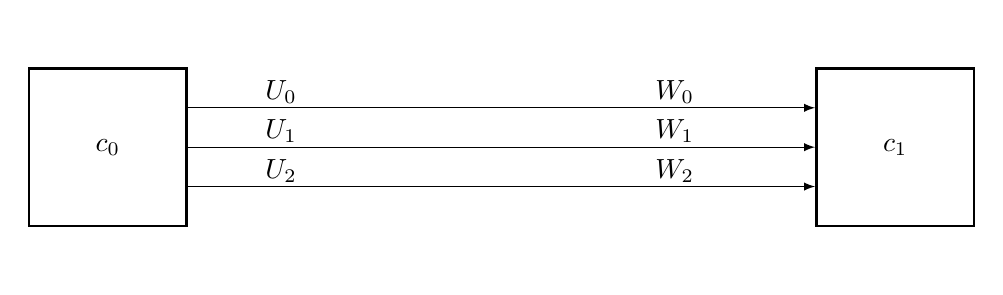
\begin{tikzpicture}
        [
            square/.style = {draw, shape=rectangle, minimum height=2cm, minimum width=2cm, node distance=2cm, line width=1pt},
            empty/.style = {draw, shape=rectangle, minimum height=2cm, minimum width=2cm, node distance=2cm, line width=1pt, draw=white},
        ]

        \node[empty] (0a) at (0,0.5)     {};
        \node[empty] (0b) at (0,-0.5)     {};
        \node[square] (0c) at (0,0)     {$c_0$};

        \node[empty] (1a) at (10cm,0.5)   {};
        \node[empty] (1b) at (10cm,-0.5)   {};
        \node[square] (1c) at (10cm,0)   {$c_1$};

        \node (x0) at (2.2cm,0.7) {$U_0$};
        \node (y0) at (2.2cm,-0.3) {$U_2$};
        \node (z0) at (2.2cm,0.2) {$U_1$};

        \node (x1) at (7.2cm,0.7) {$W_0$};
        \node (y1) at (7.2cm,-0.3) {$W_2$};
        \node (z1) at (7.2cm,0.2) {$W_1$};

        \draw [-latex] (0a.east) -- (1a.west);
        \draw [-latex] (0b.east) -- (1b.west);
        \draw [-latex] (0c.east) -- (1c.west);
    \end{tikzpicture}

}
\end{figure}

                \end{figure}
        \end{frame}

        \begin{frame}
            \frametitle{Details of Component-Based GCs (2)}
                \begin{figure}
                    \input{figure-chaining2}
                    
                \end{figure}
        \end{frame}

        \begin{frame}
            \frametitle{Efficiency of chaining garbled circuits}
            \begin{itemize}
                \item In online phase, chaining requires communicating a ciphertext per chain
                \item This can be a lot of communication
                    \begin{itemize}
                        \item Suppose $100$ by $100$ matrix with entries of max value $2^8$
                        \item Then requires $8,000$ ciphertexts
                        \item That's $256$ kBs.
                    \end{itemize}
                \item I came up with a method to reduce this to a single ciphertext per data object
            \end{itemize}
        \end{frame}

        \begin{frame}
            \frametitle{Security of Component-Based GCs}
            \begin{itemize}
                \item We think through security using a \textit{hybrid} argument.
                    \begin{itemize}
                        \item Rely on fact that computational indistinguishability is transitive
                        \item By stripping away information from the real world, we slowly transform it into the ideal world.
                    \end{itemize}
                \item We remove:
                    \begin{itemize}
                        \item Link labels
                        \item Input wire labels
                        \item Garbled tables
                        \item Output map
                    \end{itemize}
            \end{itemize}
        \end{frame}

        \begin{frame}
            \frametitle{Single Communication Multiple Connections SCMC}
            \begin{itemize}
                \item Problem: number of ciphertexts communicated scales linearly with the number of chains
                \item Key observation: 
                    \begin{itemize}
                        \item the chaining is predictable, consecutive wires are chained to consecutive wires
                        \item Pieces of data move around in a function, like matrices or numbers or text
                    \end{itemize}
                \item Solution: give consecutive wire labels a predictable pattern
            \end{itemize}
        \end{frame}


        \begin{frame}
            \frametitle{Single Communcation Multiple Connections SCMC}
            % http://tex.stackexchange.com/questions/201071/how-do-i-make-tikz-circular-arrowheads-concentric-to-the-point-they-connect
            \begin{itemize}
                \item For each piece of data, sample a label $A$.
                \item Set $i$th wire label of data to $A \oplus H(i)$.
                \item Where $H$ is a hash function
            \end{itemize}

            \begin{figure}
                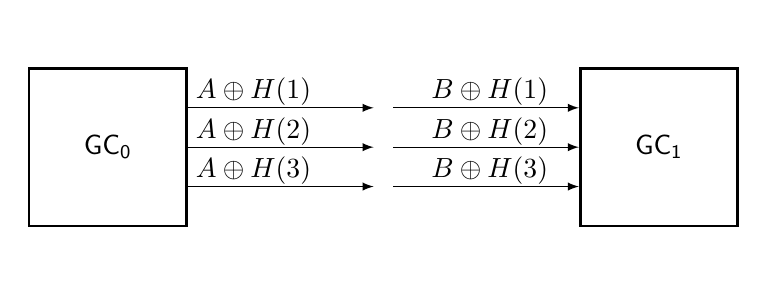
\begin{tikzpicture}
                    [
                        square/.style = {draw, shape=rectangle, minimum height=2cm, minimum width=2cm, node distance=2cm, line width=1pt},
                        empty/.style = {draw, shape=rectangle, minimum height=2cm, minimum width=2cm, node distance=2cm, line width=1pt, draw=white},
                    ]

                    \node[empty] (0a) at (0,0.5)     {};
                    \node[empty] (0b) at (0,-0.5)     {};
                    \node[square] (0c) at (0,0)     {$\GC_0$};

                    \node (mida) at (3.5cm,0.5)     {};
                    \node (midb) at (3.5cm,-0.5)     {};
                    \node (midc) at (3.5cm,0)     {};

                    \node[empty] (1a) at (7cm,0.5)   {};
                    \node[empty] (1b) at (7cm,-0.5)   {};
                    \node[square] (1c) at (7cm,0)   {$\GC_1$};

                    \node (x0) at (1.85cm,0.7) {$A \oplus H(1)$};
                    \node (y0) at (1.85cm,-0.3) {$A \oplus H(3)$};
                    \node (z0) at (1.85cm,0.2) {$A \oplus H(2)$};

                    \node (x1) at (4.85cm,0.7) {$B \oplus H(1)$};
                    \node (y1) at (4.85cm,-0.3) {$B \oplus H(3)$};
                    \node (z1) at (4.85cm,0.2) {$B \oplus H(2)$};

                    \draw [-latex] (0a.east) -- (mida);
                    \draw [-latex] (0b.east) -- (midb);
                    \draw [-latex] (0c.east) -- (midc);

                    \draw [-latex] (mida) -- (1a.west);
                    \draw [-latex] (midb) -- (1b.west);
                    \draw [-latex] (midc) -- (1c.west);
                \end{tikzpicture}
            \end{figure}
            \begin{itemize}
                \item Technically, we set the links to $A \oplus H (T \oplus (i || b))$
            \end{itemize}
        \end{frame}

        \begin{frame}
            \frametitle{Security of SCMC}
            \begin{itemize}
                \item SCMC security follows from naive component-based garbled circuits security
                \item Link labels are find to send
                \item And wire labels are \textit{pseudorandom} since $H$ is a random oracle
            \end{itemize}
        \end{frame}

        \begin{frame}
            \frametitle{Implementation}
            \begin{itemize}
                \item I implemented component-based GCs and SCMC in a program called \CompGC
                \item Written in C
                \item It does the entire garbled circuits protocol
                \item Takes circuits and inputs and securely computes the output
            \end{itemize}
        \end{frame}

        \begin{frame}
            \frametitle{Some code}
        \end{frame}

        \begin{frame}
            \frametitle{The experiments}
            \begin{itemize}
                \item AES Encryption 
                    \begin{itemize}
                        \item AES-round was only component
                    \end{itemize}
                \item CBC Mode of Operation
                    \begin{itemize}
                        \item A method for encrypting arbitrary size messages
                        \item XOR and AES-round were components
                    \end{itemize}
                \item Levensthein Distance Algorithm 
                    \begin{itemize}
                        \item Used $8$-bit alphabet
                        \item Ran 30 symbols and 60 symbols
                    \end{itemize}
            \end{itemize}
        \end{frame}

        \begin{frame}
            \frametitle{Results}
            %!TEX root = thesis.tex
\begin{table}[h]
    \tiny
    %\scriptsize
    %\small
    %\footnotesize

    \centering
    \begin{tabular}{ r c c c c c c }
        &\multicolumn{2}{c}{\textbf{Time (localhost)}}
        &\multicolumn{2}{c}{\textbf{Time (simulated network)}}
        &\multicolumn{2}{c}{\textbf{Communication}} \\
        & \Naive & \CompGC & \Naive & \CompGC & \Naive & \CompGC  \\
        \midrule
        AES
        & 4.4 $\pm$ 0.0 ms
        & 3.0 $\pm$ 0.2 ms
        & 542.6 $\pm$ 0.7 ms
        & 68.5 $\pm$ 0.2 ms
        & 24 Mb & 254 Kb \\
        CBC, 10 blocks 
        & 45.8 $\pm$ 4.0 ms
        & 22.7 $\pm$ 1.4 ms
        & 4.8 $\pm$ 0.0 s
        & 216.7 $\pm$ 0.2 ms
        & 235 Mb & 2.6 Mb \\
        Leven, 30 symbols
        & 28.9 $\pm$ 6.6 ms
        & 24.3 $\pm$ 1.2 ms
        & 2.2 $\pm$ 0.0 s
        & 315.9 $\pm$ 0.5 ms
        & 108 Mb & 6.3 Mb \\
        Leven, 60 symbols
        & 109.8 $\pm$ 7.0 ms
        & 62.2 $\pm$ 0.7 ms
        & 10.6 $\pm$ 0.0 s
        & 742.5 $\pm$ 2.0 ms
        & 524 Mb & 25 Mb \\
    \end{tabular}
    \caption[Experimental results]{Experimental results.
        Time is online computation time, not including the time to preprocess OTs, but including the time to load data from disk.
        All timings are of the evaluator's running time, and are the average of 100 runs, with the value after the $\pm$ denoting the 95\% confidence interval.
        The communication reported is the number of bits received by the evaluator.
    }
\end{table}

        \end{frame}

        \begin{frame}
            \frametitle{Results Without Loading Time}
            %!TEX root = thesis.tex

\begin{table}[h]
    \tiny
    \centering
    \begin{tabular}{ r c c c c }
        &\multicolumn{2}{c}{\textbf{Time (localhost)}}
        &\multicolumn{2}{c}{\textbf{Time (simulated network)}}\\
        & \Naive & \CompGC & \Naive & \CompGC \\
        \midrule
        AES
        & 4.4 $\pm$ 0.0 ms
        & 1.3 $\pm$ 0.1 ms
        & 542.6 $\pm$ 0.7 ms
             & 66.9 $\pm$ 0.1 ms \\
        CBC mode, 10 blocks
        & 45.8 $\pm$ 4.0 ms
        & 8.8  $\pm$ 0.5 ms
        & 4.8 $\pm$ 0.0 s
             & 204.3 $\pm$ 0.2 ms\\
        Levenshtein, 30 symbols
        & 28.9 $\pm$ 6.6 ms
        & 14.1 $\pm$ 0.4 ms
        & 2.2 $\pm$ 0.0 s
             & 305.6 $\pm$ 0.2 ms\\
        Levenshtein, 60 symbols
        & 109.8 $\pm$ 7.0 ms
        & 27.1 $\pm$ 0.4 ms
        & 10.6 $\pm$ 0.0 s
             & 703.4 $\pm$ 1.5 ms\\
    \end{tabular}
    \caption[Experimental results without loading time]{Experimental results without counting the evaluator time to load data from disk.}
    \label{tbl:results-no-load}
\end{table}

        \end{frame}

        \begin{frame}
            \frametitle{Comparing Naive to SCMC}
            %!TEX root = thesis.tex

\begin{table}[h]
    %\small
    \scriptsize
    \centering
    \begin{tabular}{ r c c c c }
        &\multicolumn{2}{c}{\textbf{Time (simulated network)}}
        &\multicolumn{2}{c}{\textbf{Communication}} \\
        & Standard & \scmc & Standard & \scmc \\
        \midrule
        AES
        & 134.4 $\pm$ 0.1 ms
        & 68.5 $\pm$ 0.2 ms
        & 656 Kb & 254 Kb \\
        CBC mode, 10 blocks 
        & 321.5 $\pm$ 0.9 ms
        & 216.7 $\pm$ 0.2 ms
        & 7.4 Mb & 2.6 Mb \\
        Levenshtein, 30 symbols
        & 371.0 $\pm$ 0.9 ms
        & 315.9 $\pm$ 0.5 ms
        & 10.0 Mb & 6.3 Mb \\
        Levenshtein, 60 symbols
        & 1119.6 $\pm$ 2.1 ms
        & 742.5 $\pm$ 2.0 ms
        & 44 Mb & 25 Mb \\
    \end{tabular}
    \caption[Comparison of naive protocol to SCMC]{Comparison of the two approaches for component-based garbled circuits: the standard approach and the \scmc approach.
    The experiments are run on the simulated network.}
    \label{tbl:results-scmc}
\end{table}

        \end{frame}

        \begin{frame}
            \frametitle{Future work}
            \begin{itemize}
                \item Malicious setting
                \item MPC - more than two parties
                    \begin{itemize}
                        \item Then we can do auctions and elections with arbitrarily many parties
                    \end{itemize}
                \item Make linking faster
                \item Reduce memory footprint
                \item Develop a library of components
            \end{itemize}
        \end{frame}

    \end{document} 






